\section{Experimental results}
In this section we present experimental results for the simplicial neural network. The datasets we analyze have been extracted from the Semantic Scholar datasets. The data consists of XXX papers together with their authors and number of citations. We retain paper with more than $5$ citations and at most $10$ authors.

An important step in preprocessing many kinds of input data in TDA is constructing a simplicial complex. Our work focus on \emph{collaboration complexes} (or \emph{co-authorship complexes}) \stefania{cite paper Alice}, simplicial complexes where a paper with $k$ authors is represented by a $(k-1)$-simplex. We constructed different co-authorship complexes by considering sub-samplings from the papers set of the Semantic Scholar dataset. The sub-samplings were obtained by performing random walks on the nodes of the graph which vertices corresponds to the papers and edges connect papers sharing at least one author. The co-authorship complexes obtained from each sub-sampling  have corresponding $k$ co-chain given by the number of shared citations.

We evaluate the performance of the SNN on the task of predicting missed input data. 
Specifically, given a fixed co-authorship complex missing data is introduced 
at random on the training co-chains at $4$ levels: $10\%,  20\%,  30\%$, and $50\% $.   As in a typical pipeline for this task, in our approach missing data is first replaced by some values. In our case the training input is given by the citations on the co-authorship complex where the random missing data is substituted by the median of the known data. We trained a SNN composed by $3$-layers with $30$ convolutional filters of degree $5$. We used the $L_1$ norm as reconstruction loss over the known elements an the Adam optimizer with learning rate of $1\times 10^{-3}$. The SNN was trained for $1000$ iterations. We then test the performance of the network on its accuracy in predicting the missing data. A predicted citation is considered correct if the predicted value differs of at most $1$ from the actual number of citations. The prediction error is the absolute value of the difference between the predicted citation and the actual value of the citation. 

Figure~\ref{fig:accuracy} shows the accuracy of the SNN in prediction missing citations on CC1 (Co-authorship Complex 1, Table~\ref{table:Simplices-coauthor}). The distribution of the prediction error is shown in Figure~\ref{fig:error}. 
\begin{table}
  \caption{%
  Number of simplices
  }
  \label{table:Simplices-coauthor}
  \centering
  \begin{tabular}{llllllllllll}
    \cmidrule(r){1-12}
    Dimension   & 0     & 1  & 2     & 3 & 4     & 5 & 6    & 7 & 8   & 9 & 10\\
    \midrule
    CC1 & 352  & 1474  & 3285  & 5019  & 5559  & 4547  & 2732  & 1175  & 343 & 61 & 5\\
    CC2 & 1126 & 5059 & 11840 & 18822 & 21472 & 17896  & 10847 & 4673 & 1357 & 238 & 19\\ 
    \bottomrule
  \end{tabular}
\end{table}
%\begin{figure}[htbp]
%  \centering
 
%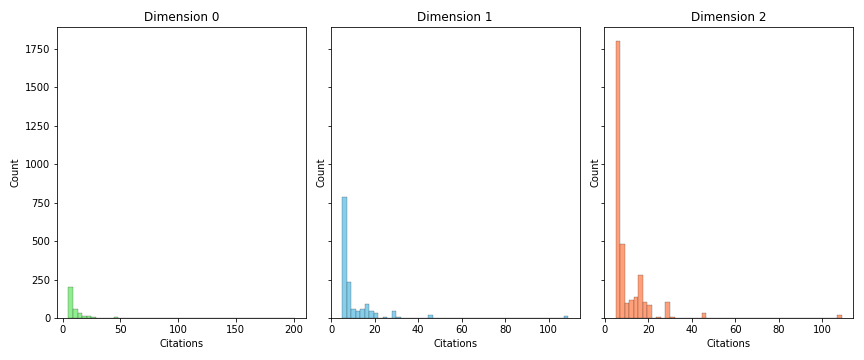
\includegraphics[scale=0.35]{./figures/distribution_cohain_150250.png}
% \caption{Distribution of the citation in CC1 } \label{fig:accuracy}
%\end{figure}
\begin{figure}[htbp]
  \centering 
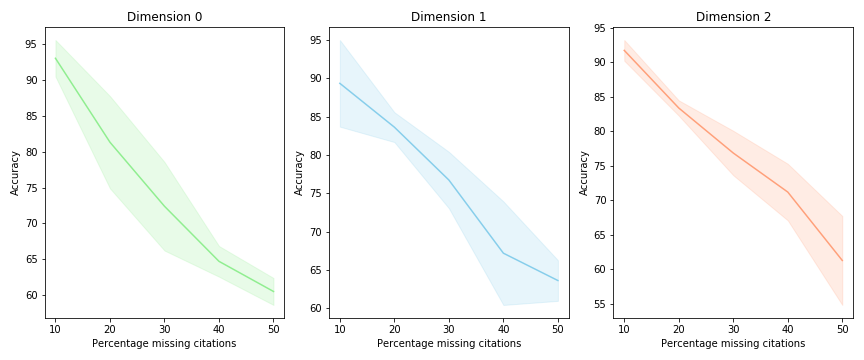
\includegraphics[scale=0.4]{./figures/accuracy_network1.png}
 \caption{Accuracy of SNN in predicting missing citations } \label{fig:accuracy}
\end{figure}
\begin{figure}[htbp]

  \centering
 \hspace{-6cm}
 
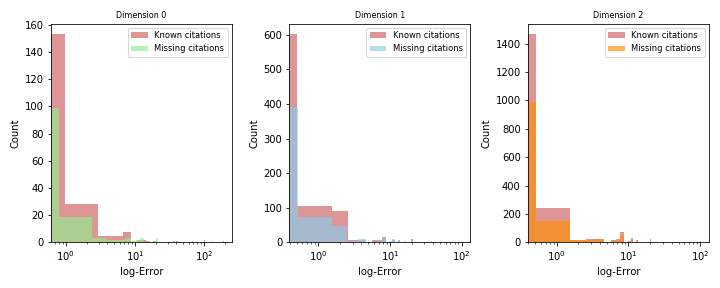
\includegraphics[scale=0.4]{./figures/Error_dist_start150250_seed6666_notsee40.png}
  \caption{Distribution of the prediction's error} \label{fig:error}
\end{figure}

As a second assessment of our network we use transfer learning . In particular, we test how accurately a SNN pretrained on a co-authorship complex can predict citations on a different complex. Figure shows the test accuracy on predicting missing values of the SNN on CC2 (Co-authorship Complex 2, see Table~\ref{table:Simplices-coauthor}) and evaluate in predicting the missing values of CC1.

\stefania{Say computations are done up to dimension 3}


\begin{figure}[htbp]
  \centering
 
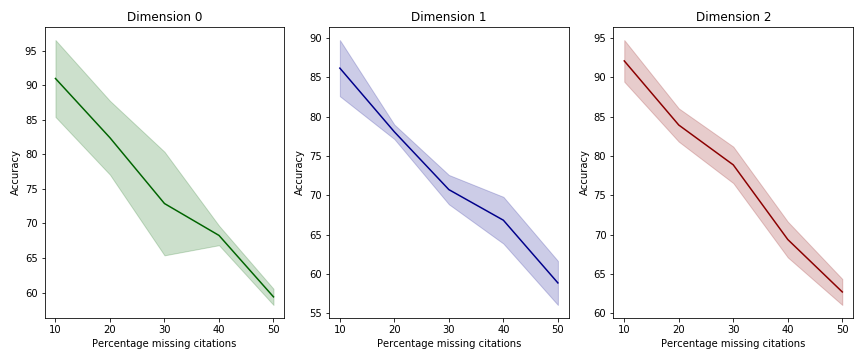
\includegraphics[scale=0.4]{./figures/accuracy_network1_pretrained.png}
  \caption{Accuracy in predicting missing citations with a pretrained SNN }
\end{figure}

